% This is a semi-simple sample document.

\documentclass{article} % Define the type of document

% Package imports for additional functionality
\usepackage{mathtools} % Enhanced math functionality (includes amsmath)
\usepackage{amssymb} % Additional math symbols
\usepackage{graphicx} % Image package
\usepackage{float} % Float specifiers for figures and tables
\usepackage{subcaption} % Subfigures
\usepackage[margin=1in]{geometry} % Set page margins
\usepackage{chngcntr} % For section-specific figure numbering
\usepackage{setspace} % Set line spacing
\usepackage{appendix} % Appendices
\usepackage[hidelinks]{hyperref} % Hyperlinks without borders
\usepackage{algorithm} % For algorithm environment
\usepackage{algorithmic} % For algorithmic commands

% Customize figure numbering
\counterwithin{figure}{section}

% Title, author, and date information
\title{Semi-Simple Sample Document}
\date{November 2021}
\author{
    Matías Loiseau\\
    Departamento de Tecnología y Administración\\
    Ingeniería en Informática\\
    \texttt{mloiseau@undav.edu.ar}
    \and
    Jon Snow\\
    Winterfell University\\
    \texttt{jsnow@winterfell.edu.ar}
}

% Begin document
\begin{document}

\begin{figure}
    \centering
    
\includegraphics[width=0.2\textwidth]{images/undav-logo}
    \caption{University Logo}
    \label{fig:undav-logo}
\end{figure}

\maketitle % Create title using information in preamble
\thispagestyle{empty} % Suppress page number on title page
\clearpage

\tableofcontents % Generate table of contents
\clearpage

\section{Forms to Write Text} % Creates a section
Normal text.

\textbf{Text in bold (Ctrl + B)}

\textit{Text in italic (Ctrl + I)}

Text with a footnote\footnote{This is a footnote.}

This is a citation\cite{knn}.

\subsection{Enumerate and Itemize Information}

\begin{enumerate}
    \item Enumerate one
    \item Enumerate two
    \begin{enumerate}
        \item Sub-enumerate one
        \item Sub-enumerate two
    \end{enumerate}
\end{enumerate}

\begin{itemize}
    \item Item one
    \item Item two
    \begin{itemize}
        \item Sub-item one
        \item Sub-item two
    \end{itemize}
\end{itemize}

\begin{enumerate}\setcounter{enumi}{0}
    \item Start enumeration at 0
    \item Enumerate one
\end{enumerate}

\section{Spaces}

Add space between \quad words.

Carbon monoxide (CO) is a colorless, odorless, and tasteless gas composed of one carbon atom and one oxygen atom. It is produced through incomplete combustion of carbon-containing fuels such as gasoline, natural gas, coal, wood, and oil. When these fuels do not burn completely due to insufficient oxygen supply, carbon monoxide is formed instead of carbon dioxide (CO\textsubscript{2}).

\begin{spacing}{0.8} 
Carbon monoxide (CO) is a colorless, odorless, and tasteless gas composed of one carbon atom and one oxygen atom. It is produced through incomplete combustion of carbon-containing fuels such as gasoline, natural gas, coal, wood, and oil. When these fuels do not burn completely due to insufficient oxygen supply, carbon monoxide is formed instead of carbon dioxide (CO\textsubscript{2}).
\end{spacing}

\begin{spacing}{1.5} 
Carbon monoxide (CO) is a colorless, odorless, and tasteless gas composed of one carbon atom and one oxygen atom. It is produced through incomplete combustion of carbon-containing fuels such as gasoline, natural gas, coal, wood, and oil. When these fuels do not burn completely due to insufficient oxygen supply, carbon monoxide is formed instead of carbon dioxide (CO\textsubscript{2}).
\end{spacing}

\section{Equations}

\subsection{Simple Equations}

\begin{equation}
    E=mc^2
\end{equation}

\begin{equation}
    f(x) =
    \begin{cases*}
        1 & if $x > 0$\\
        0 & if $x \leq 0$
     \end{cases*}
\end{equation}

\subsection{Complex Equations}

\begin{align}
    \vec{h}_1 &= f(\vec{x} \cdot W_1) \label{eq:layers1} \\
    \vec{h}_2 &= f(\vec{h}_1 \cdot W_2) \\
    \vec{h}_3 &= f(\vec{h}_2 \cdot W_3) \\
    \vec{y} &= f(\vec{h}_3 \cdot W_4)
\end{align}

\begin{equation}\label{eq:mse}
    \text{MSE} = \frac{1}{n} \sum_{i=1}^{n}(y_{i} - \hat{y}_{i})^2
\end{equation}

\[
\begin{pmatrix} a_0 & a_1\\ a_2 & a_3 \end{pmatrix}
\odot
\begin{pmatrix} b_0 & b_1\\ b_2 & b_3 \end{pmatrix}
=
\begin{pmatrix} a_0 \cdot b_0 & a_1 \cdot b_1\\ a_2 \cdot b_2 & a_3 \cdot b_3 \end{pmatrix}
\]

\[
\frac{dL}{db_k} = \frac{dL}{dy_k} \frac{dy_k}{db_k} = \frac{dL}{dy_k} \frac{dy_k}{dz_k} \frac{dz_k}{db_k} = l'_{k+1} \odot f'_k \frac{d(W_k x_k + b_k)}{db_k}
\]

\subsubsection{Matrix}

\begin{equation}
    \text{IoU}(A,B) = \frac{|A \cap B|}{|A \cup B|} = \frac{|A \cap B|}{|A| + |B| - |A \cap B|}
\end{equation}

\clearpage

\section{Figures}

\begin{figure}[H]
    \centering
    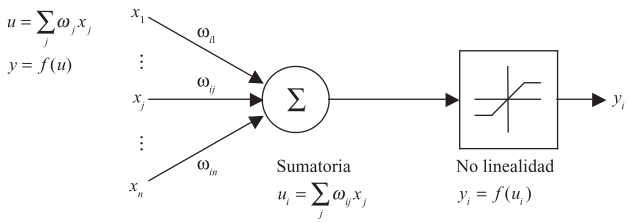
\includegraphics[width=0.8\textwidth]{images/perceptron-graph}
    \caption{Perceptron diagram.}
    \label{fig:perceptron-graph}
\end{figure}

This is a reference for the image (Figure \ref{fig:perceptron-graph}) above.

\begin{figure}[H]
    \centering
    \begin{subfigure}{0.45\textwidth}
        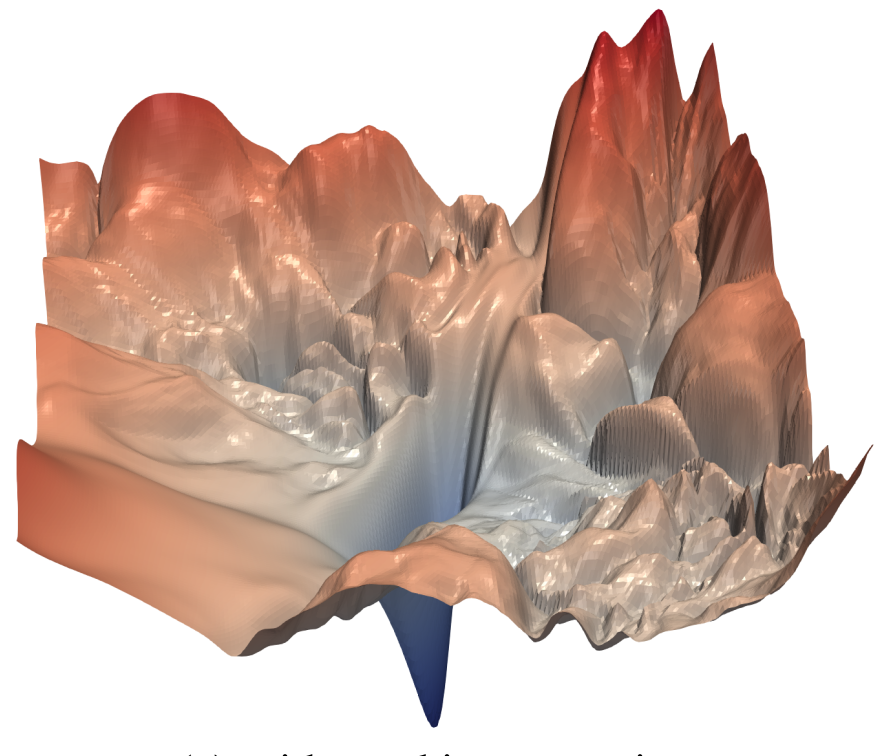
\includegraphics[width=\linewidth]{images/mse-visu-1}
        \caption{Figure one.}
        \label{fig:mse-visu-1}
    \end{subfigure}    
    \hfill
    \begin{subfigure}{0.45\textwidth}
        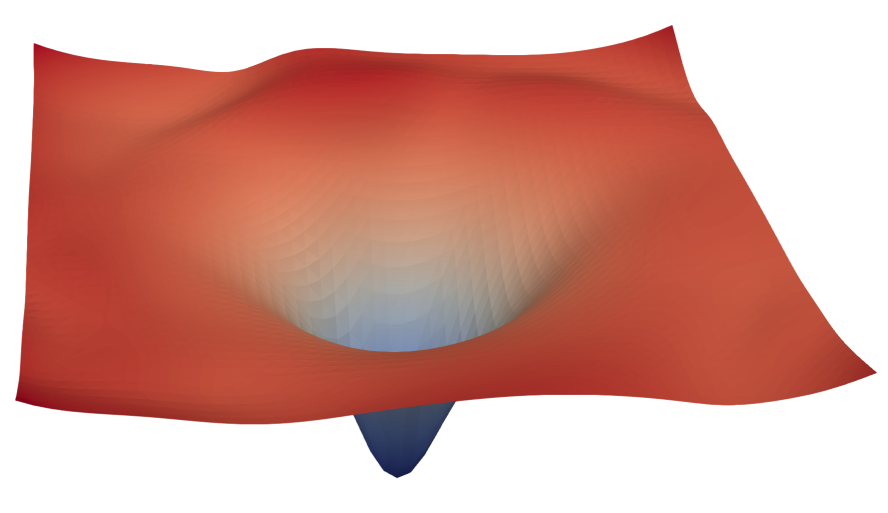
\includegraphics[width=\linewidth]{images/mse-visu-2}
        \caption{Figure two.}
        \label{fig:mse-visu-2}
    \end{subfigure}
    \caption{Both figures.}
    \label{fig:mse-visu-12}
\end{figure}

\section{Tables}

\begin{table}[H]
    \centering
    \begin{tabular}{||l | c ||}
        \hline\hline
        Data 1 & 185\\
        \hline
        Data 222 & 37\\
        \hline
        Data 333333 & 12\\
        \hline
        Data 4444444444 & 12\\
        \hline
        Data 555 & 13\\
        \hline\hline
    \end{tabular}
    \caption{Table X.}
    \label{tab:table-x}
\end{table}

\begin{table}[H]
    \centering
    \begin{tabular}{||l || c | c | c | c | c ||}
        \hline\hline
        & \multicolumn{3}{c|}{Number of people} & \multicolumn{2}{c||}{Difference between}\\
        \hline
        Module & 0 & 1 & 2 & 1 vs 0 & 2 vs 0\\
        \hline\hline
        1 & 21.07 & 21.19 & 21.33 & 0.12 & 0.26\\
        \hline
        2 & 22.25 & 22.35 & 22.39 & 0.10 & 0.14\\
        \hline
        3 & 18.11 & 18.19 & 18.61 & 0.07 & 0.50\\
        \hline
        4 & 18.30 & 18.44 & 18.87 & 0.15 & 0.57\\
        \hline
        6 & 18.21 & 18.43 & 19.45 & 0.21 & 1.24\\
        \hline\hline
    \end{tabular}
    \caption{Table Y.}
    \label{tab:table-y}
\end{table}

\section{Algorithm Example}

Using the `algorithm` and `algorithmic` packages.

\begin{algorithm}[H]
\caption{Example Algorithm: Binary Search}
\label{alg:binary-search}
\begin{algorithmic}[1]
\REQUIRE Sorted array $A[1 \dots n]$, target value $x$
\ENSURE Index of $x$ in $A$, or -1 if not found
\STATE $low \gets 1$
\STATE $high \gets n$
\WHILE{$low \leq high$}
    \STATE $mid \gets \lfloor (low + high) / 2 \rfloor$
    \IF{$A[mid] = x$}
        \RETURN $mid$
    \ELSIF{$A[mid] < x$}
        \STATE $low \gets mid + 1$
    \ELSE
        \STATE $high \gets mid - 1$
    \ENDIF
\ENDWHILE
\RETURN $-1$
\end{algorithmic}
\end{algorithm}


\clearpage

\appendix
\appendixpage
\addappheadtotoc

\section{First Appendix}\label{app:one}

This is an appendix.

\clearpage

\section{Second Appendix}\label{app:two}

Text.

\clearpage

\begin{thebibliography}{9}
\addcontentsline{toc}{section}{Bibliography}

\bibitem{iot}
Iván Federico Kwist, Matías Loiseau, David Exequiel Contreras, Federico Gabriel D’Angiolo, Roberto Osvaldo Mayer. (2019). \textit{Monitorización de un Datacenter mediante Protocolos de IoT}. Congreso Nacional de Ingeniería Informática – Sistemas de Información.

\bibitem{regresion-lineal}
Federico Gabriel D’Angiolo, Iván Federico Kwist, Matías Loiseau, David Exequiel Contreras, Fernando Asteasuain. (2019). \textit{Algoritmos de Regresión Lineal aplicados al mantenimiento de un Datacenter}. Congreso Argentino de Ciencias de la Computación.

\bibitem{knn}
Federico Gabriel D’Angiolo, Iván Federico Kwist, Matías Loiseau, David Exequiel Contreras, Gregorio Oscar Glas. (2019). \textit{Algoritmo de KNN aplicado al mantenimiento de un Datacenter}. Congreso Nacional de Ingeniería Informática – Sistemas de Información.

\bibitem{deep-learning-nature}
LeCun, Y., Bengio, Y., \& Hinton, G. (2015). \textit{Deep learning}. Nature, 521(7553), 436-444.

\bibitem{object-detection-review}
Zhao, Z. Q., Zheng, P., Xu, S. T., \& Wu, X. (2019). \textit{Object detection with deep learning: A review}. IEEE Transactions on Neural Networks and Learning Systems, 30(11), 3212-3232.

\end{thebibliography}

\end{document} % End of the document
